\documentclass{article}

\usepackage[utf8]{inputenc}
\usepackage[T1]{fontenc}
\usepackage{graphicx}

\begin{document}

\begin{flushright}
Błażej Pawluk, 279738
\end{flushright}

\title{WSI, Laboratorium, Lista 2}
\date{}
\maketitle

\section*{Układanka 3x3}
Heurystyka niepoprawnych pol:
Srednia ilosc odwiedzonych stanow: 13866.038
Srednia ilosc ruchow potrzebnych do rozwiazania: 23.296

Heurystyka manhattan:
Srednia ilosc odwiedzonych stanow: 1186.416
Srednia ilosc ruchow potrzebnych do rozwiazania: 23.296

\section*{Układanka 4x4}

\begin{figure}[h!]
	\centering
	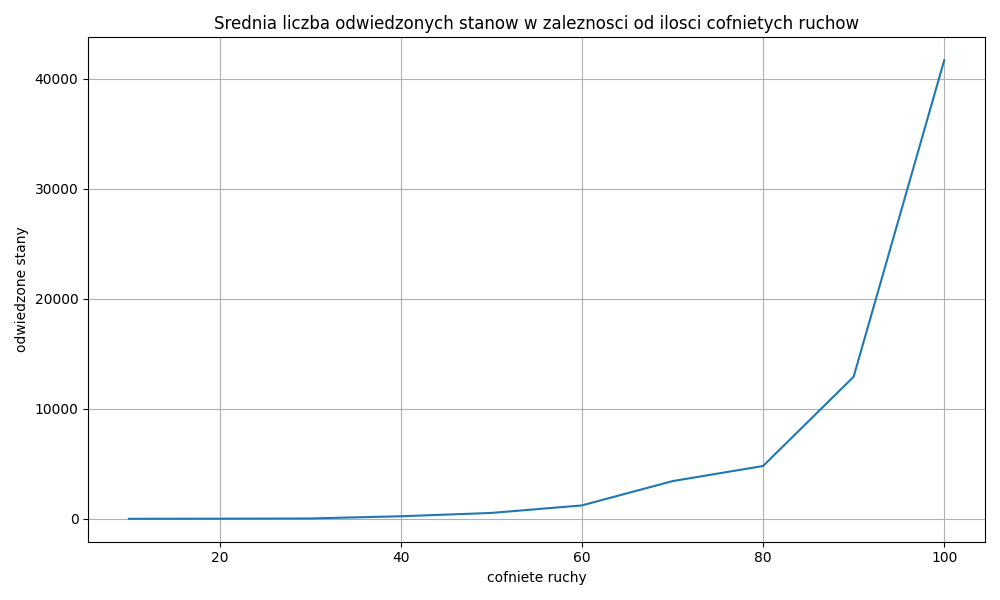
\includegraphics[width=1\textwidth]{images/stany.png}
	\caption{}
\end{figure}

\begin{figure}[h!]
	\centering
	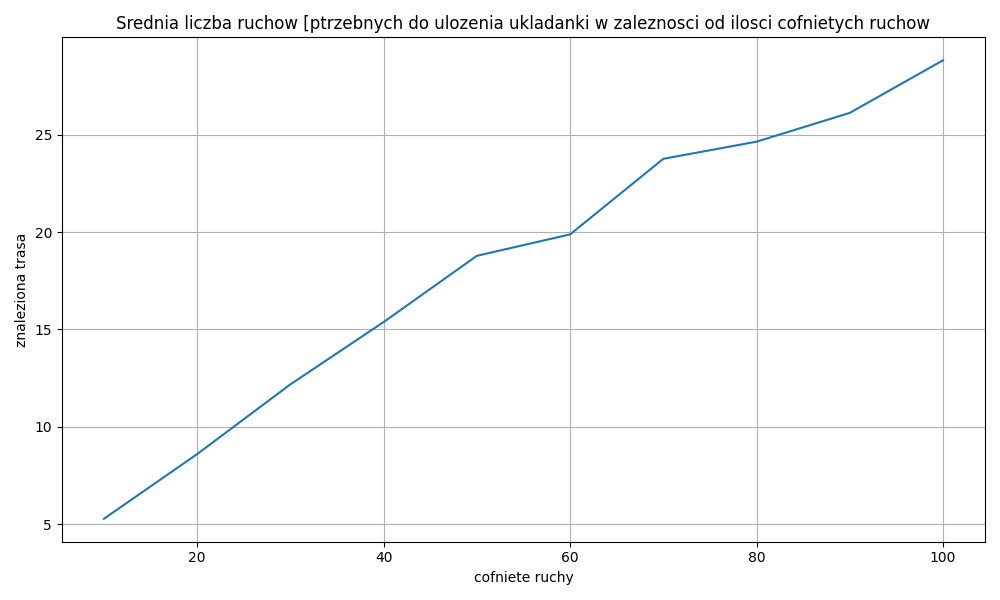
\includegraphics[width=1\textwidth]{images/trasa.png}
	\caption{}
\end{figure}

\end{document}